\subsection{Formal ontologies}

Formal ontologies are centred on classes of individual entities. Together with a set of binary relations and operators in a logic-based language such as a DL dialect, they constitute formal axioms. Axioms are limited to statements about what is universally true for all members of a class or a class-like expression, e.g. that all nucleic acid molecules contain nucleotides, or that all adenine molecules are nucleotides. The construction of (formal) ontologies should obey principled criteria \citep{Spear2006} and good practice guidelines \citep{Schulz2012}. Important principles are (i) naming conventions \citep{Schober2009}; (ii) mutually disjoint upper-level classes like \emph{Process} or \emph{Quality} as a fundamental ordering framework; and, (iii) a limited set of canonical relations \citep{Smith2005}. 

We distinguish \emph{ontology content} properly from both the notions of \emph{knowledge} \citep{Naturwissenschaften2014} and \emph{data}. Knowledge, in a broader sense \citep{Rector2008}, emcompasses assertions about what is frequently associated or what is true by default. This is beyond the scope of formal ontologies. Data, in contrast, are first of all information entities in a database. Like words in a text, data elements constitute denoting entities. 
%Their interpretation is often blurred by use-mention confusion, i.e. mixing data items with the things they denote. 
In databases, the interpretation of data elements is determined by the use cases embedded in the underlying schema. The distinction between what is a data element and what is denoted by it is often neglected and leads to use-mention confusions. Formal ontologies must enforce this distinction: 
all data items are instances of a specific class like \textit{information object} in BTL2, or \textit{generically dependent continuant} in BFO, whereas the things data items denote are manifold: individuals, classes, or even nothing \citep{Schulz2011a}.

%Formal ontologies present mostly extensive (poly-) hierarchies of representational units, named classes, related by a limited set of binary relations. Ontologies are centred around classes. Together with a set of binary relations and logical operators in a logic-based language, e.g., DL, they constitute formal axioms.  Axioms state what is universally true for all members of a class or a class-like expression. For instance, all nucleic acid molecules contain nucleotides, or all adenine molecules are nucleotide molecules.
%
%The construction of (formal) ontologies should obey principled criteria \citep{Spear2006} and good practice guidelines \citep{Schulz2012}. Important principles are (i) naming conventions \citep{Schober2009}; (ii) mutually disjoint upper-level classes like Process or Quality as a fundamental ordering framework; and, (iii) a generally small set of canonical relations \citep{Smith2005}, such as ‘has participant’ or ‘has part’. Both top-level classes and canonical relations are usually supplied by top-level ontologies, such as BFO \citep{Spear2006}, RO \citep{Smith2005}, or BTL2.
%
%We distinguish ontology content properly from both the notions of knowledge (Schulz and Jansen, 2013) and data. Regarding knowledge\footnote{In a broader sense, Cf. \citep{Rector2008}}, assertions about what is frequently associated or only true by default can- not be straightforwardly expressed by formal ontologies. Regarding data, interpretation is often blurred by use-mention confusion, i.e. mixing data items with the things they denote. In databases, the interpretation of data elements is determined by the use cases embedded in the underlying schema. The distinction between what is a data element and what is its referent is often implicit. Formal ontologies should enforce this distinction: data items are instances of information content entities, whereas the things data items denote are manifold: individuals, classes, or even nothing\citep{Schulz2011a}.

\subsection{Interpreting databases with ontologies}
Databases and less-principled domain ontologies leave the real nature of the entities as well as and the circumstances of denotation underspecified, assuming that this is intuitively known by the users and interpreted accordingly within the expected context of use. An example is ``Human", which may denote an individual person, the class \textit{Homo sapiens}, the quality of an object belonging to the taxon \textit{Homo sapiens} \citep{Schulz2008}, or a population of humans. In a similar vein, ``Animal" could be interpreted as including the class \textit{Homo sapiens}, in the context of Biology or excluding it, e.g. in the context of Law. Such ambiguities underline the need to make hidden assumptions explicit, which is the main rationale for the ontological grounding mechanism as described in the following. 
Content retrieval applications that use existing domain ontologies as vocabularies, like the ones derived from OBDA might benefit from this. As ODBA tools are unable to retrieve and generate new ontology content, the interpretation goes beyond what the user has specified as task-specific mappings between databases and ontologies. This requires that databases do not only use domain ontologies as standardized vocabularies, but that the meaning of their entire structure and content is described by ontology axioms and assertions. This is what we propose.

\subsection{Description Logics and OWL2}

Description Logics (DLs) are representation languages used to formalise ontology content\footnote{For DL syntax and semantics, Cf. \cite{Baader2007g}.}. DL classifiers, like Fact++ \citep{Tsarkov2006}, find new subclass links, identify equivalent classes, and assure satisfiability, by spotting contradictory axioms. An important distinction of ontology content is between ABox and TBox. TBoxed are constituted by class level axioms (e.g., ``all chimps are primates"),  whereas ABoxes contain assertions on individuals (e.g., ``Washoo is a chimp").

The Semantic Web Standard OWL2 \citep{W3C2012} uses the DL language $SROIQ$ \citep{Horrocks2006}, with limited expressiveness but complete and finite reasoning. OWL2 supports classes, binary relations (called object properties), and individuals, together with related axioms and assertions. For instance, the OWL2 class \textit{Drosophila melanogaster} has all individual fruit flies as members. Because all individual fruit flies are also members of the class \textit{Organism}, the class  \textit{Drosophila melanogaster} forms a subclass of the class \textit{Organism}. 
% iff all particular drosophila are equally members of \textit{Organism}.
Such class statements are constructed  by the combination  of operators specified in OWL2; \emph{viz}. `and' for conjunctions, `or' for disjunctions, `some' for existential restrictions, and `only' for value restrictions, under the Manchester Syntax for OWL2 \citep{Horridge2009}, which we will use in this paper. 



%Description Logics (DLs) are representation languages used to formalise ontology content. DL classifiers, like HermiT \citep{Glimm2014}, find new subclass links, identify equivalent classes, and assure satisfiability, by spotting contradictory axioms. TBox expressions are class level axioms (e.g., ``all chimps are primates"), whereas ABox contain assertions on individuals (e.g., ``Washoo is a chimp").
%
%The Semantic Web Standard OWL2 \citep{W3C2012} uses the DL language $SROIQ$ \citep{Horrocks2006}, with limited expressiveness but complete and finite reasoning. OWL2 supports classes, binary relations (called object properties), and individuals, together with related axioms and assertions. For instance, the OWL2 class `\textit{Drosophila melanogaster}' has all individual drosophila as members. As all individual drosophila are members of \textit{Organism}, we can infer taxonomic subsumption: `\textit{Drosophila melanogaster}' forms a subclass of \textit{Organism} iff all particular drosophila are equally members of \textit{Organism}.
%
%Such class statements are constructed by the combination of operators specified in OWL2, viz. `and' for conjunctions, `or' for disjunctions, `some' for existential restrictions, and `only' for value restrictions, under the Manchester Syntax for OWL2 \citep{Horridge2009}\footnote{In this work,  classes are written  in \textit{italic}, binary relations (OWL object properties) in \textbf{bold} case.}.

\subsection{Application background}

For the use  case,  we use data  and ontologies  related to the metabolism of homocysteine (Hcy). Hcy is an amino acid, which plays  a key role in vitamin and cofactor  metabolism,  neuronal metabolism,  and in the biological oxidation of enzymes \citep{Selhub1999}. 
%Hcy is also involved  in the metabolism of sulphur-based amino acids, where it can be converted into methionine or cysteine (Vitamin B6 dependent).  When converted into methionine,  the reaction depends on cobalamin (Vitamin B12) and requires 5-methyltetrahydrofolate (5-methyl-THF) \citep{Selhub1999}.
%For the use case, we use data and ontologies related to the metabolism of homocysteine (Hcy). Hcy is an amino acid, which plays a key role in vitamin and cofactor metabolism, neuronal metabolism, and in the biological oxidation of enzymes. Hcy is also involved in the metabolism of sulphur-based amino acids, where it can be converted into methionine or cysteine (Vitamin B6 dependent). When converted into methionine, the reaction depends in cobalamin (Vitamin B12) and requires 5-methyltetrahydrofolate (5-methyl-THF) \citep{Selhub1999}. 
%
%The latter is result of the reduction of 5,10-methyl-THF via 5,10-methyl-THF reductase, an enzyme that regulates Hcy levels \citep{Selhub1999}. 
High levels of Hcy are reported to play a role in the pathogenesis of atherosclerosis \citep{Muniz2006}, and of hepatic steatosis in hepatitis C infected subjects \citep{Siqueira2011b}. Many organisms host Hcy-related bioprocesses, e.g. \textit{Mus musculus}, \textit{Homo sapiens}, \textit{Gallus gallus}, \textit{Schizosaccharomyces pombe}, and \textit{Oryza sativa}.

\subsection{Ontology grounding}
% MUST BE A SUBSECTION, NOT A SECTION
Ontology grounding means the detailed description of database structure and content by formal ontology mechanisms. This process requires in-depth domain knowledge, insight into the way databases are populated, as well as ontology engineering skills, based on the understanding of upper level ontology principles and description logics.
Aware that a straightforward,  automatized ``ontologization'' of a database schema is not sufficient, the ontology engineer has to critically assess the pros and cons of competing modelling strategies, in a way that correctly accounts for the underlying domain segment, and which provides enough expressiveness to address typical queries (Fig. \ref{fig:process}). 

This grounding process starts with the identification of typical domain-related queries and their definition as Competency Questions (CQs) \citep{Gruninger1994}. Then databases that are needed to answer these CQs are selected, as well as the ontologies that are referred to by these databases. Ontology annotations in databases as well as database structure and content are identified and linked to the ontology entities they denote, which can be TBox or ABox entities. 

Top-level classes and relations of the domain ontologies are mapped to an upper level ontology. During this mapping process, consistency is iteratively checked by a DL reasoner. Repetitive structures are identified in database records according to the ontology organization and described as generalizable ontology design patterns. In this process, the interdependencies and relationships between the referents and/or their types are analysed, based on domain knowledge, and the need for newly defined subclasses is assessed. 

General patterns are applied to the overall databases or to database subsets under consideration and are formatively evaluated by test queries that were formulated beforehand. When the content generated is logically consistent and the answers to the test queries are complete, the process reaches the end, and the output corresponds to an ontologized interpretation of the database. Otherwise, more iterations and evaluations are required in order to meet consistency, domain validity and user expectations. 
  
\begin{figure}[h]
\centering
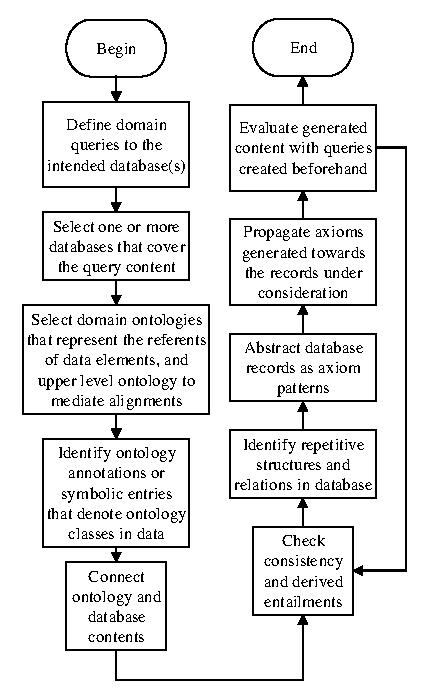
\includegraphics{./PIC/process}
\caption{Ontology grounding process.}
\label{fig:process}
\end{figure}

For assessment and demonstration of the ontology grounding approach we have formulated the following CQs on Hcy metabolism. They explore database content concerning phenotypes, proteins, molecules and biological processes from several organisms, using ontologies and databases described in Section \ref{sec:resources}).

\begin{enumerate}
	\item Which kinds of biological processes related to Hcy can be found in mice?
	\item Which are the proteins that exhibit  \textit{methyltransferase activity}? 
	\item Which are the kinds of biological processes in which proteins of the type \textit{cystathionine gama lyase} participate, exhibiting \textit{carbon-sulfur lyase activity}?
	\item Which dysfunctional biological processes entail a risk of \textit{Myocardial infarction}?
	\item Which kinds of organisms are capable of performing `\textit{cysteine biosynthetic process}'?
	\item Which proteins found in ruminants have the capability of methionine biosynthesis? 
\end{enumerate}


